\section{Circuit Design \& Electronics}

\subsection{Components Selection \& Justification}

Every electronic component for this project was chosen through a structured evaluation against four consistent criteria: technical fit with the system architecture, library and toolchain support, compatibility with Tunisian operator networks where applicable, and local availability in Tunisia together with unit cost.

\paragraph{Microcontroller --- ESP32-DEVKITC.}
The MCU is the brain of the ISS board. It must handle CAN data acquisition, sensor reading, GPRS connectivity, and real-time telemetry transmission simultaneously. The ESP32 integrates Wi-Fi, Bluetooth, and a dedicated UART for the GPRS module in a single chip, removing the need for extra communication modules~\cite{esp32datasheet}. Its compatibility with the Arduino IDE and the large IoT library ecosystem significantly accelerated development. The WROOM module is widely available locally in Tunisia and costs approximately 30~TND, making it the most practical and cost-effective choice.

\paragraph{CAN Controller --- MCP2515.}
The CAN controller acts as the interface between the ESP32 and the vehicle CAN bus. Three options were evaluated: the ESP32's built-in TWAI peripheral, the legacy SJA1000, and the MCP2515. Although the ESP32 includes a built-in CAN peripheral, it is only accessible through the ESP-IDF framework, making it significantly harder to integrate with Arduino-style libraries. The MCP2515 communicates over SPI, keeping wiring simple and reliable~\cite{mcp2515datasheet}. Its well-documented \texttt{mcp\_can} library and local availability in Tunisia made it the most practical choice. Three MCP2515 SPI module headers (J17, J18, J19) are present on the board to support multi-bus configurations.

\paragraph{CAN Transceiver --- TJA1051T.}
The CAN transceiver translates the digital logic signals from the MCP2515 into the differential voltage levels required on the physical CAN bus~\cite{iso11898}. The TJA1051T is an automotive-grade transceiver that operates at 5~V, directly matching the MCP2515 supply rail~\cite{tja1051datasheet}. It provides robust bus fault protection suited for the electrically noisy environment of a vehicle. It is the standard companion chip to the MCP2515 in OBD and automotive data-logging applications, ensuring long-term reliability.

\paragraph{Cellular Module.}
The SIM800L relies on 2G connectivity, which is being progressively phased out by Tunisian operators, making it a short-lived solution. The SIM800L supports 4G GPRS Cat-M1 and NB-IoT, is confirmed compatible with both Ooredoo and Orange networks in Tunisia, and remains future-proof as the country's network infrastructure continues to evolve. Its low operating cost further justified this selection. The KiCad schematic uses the SIM800L-CORE footprint as a physical layout placeholder; the component actually populated on the board is the SIM800L as noted in Section~\ref{sec:components-inventory}.

\paragraph{Power Regulation.}
The board is powered from the vehicle's 12~V rail. The LM2596S-ADJ is a switching buck regulator capable of delivering up to 3~A with approximately 90\% efficiency, producing minimal heat compared to a linear regulator~\cite{lm2596datasheet}. Its adjustable output (1.25~V to 37~V) allows the same component to supply both the 3.3~V ESP32 circuit and a 5~V rail. The board also carries an AMS1117 (V3.3) and an LM7805 (V5) for localised regulation where switching noise is undesirable.

\subsection{Circuit Schematic Description}

\begin{figure}[H]
    \centering
    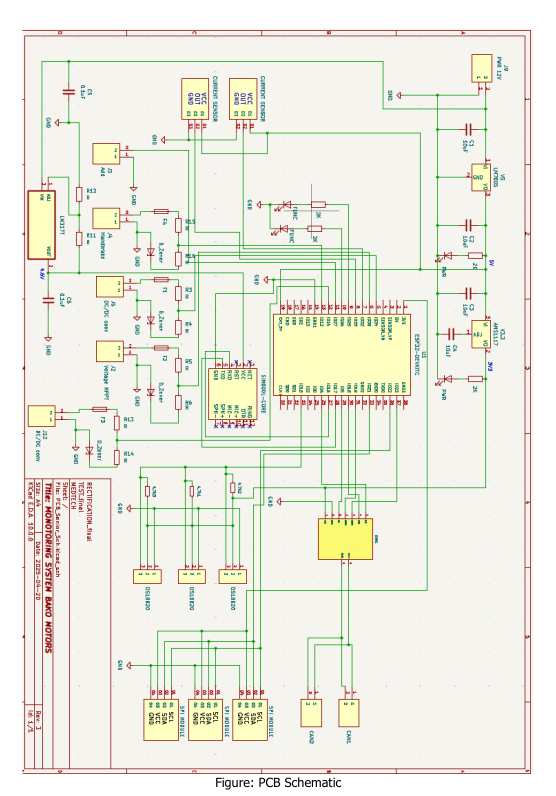
\includegraphics[width=\textwidth]{images/schematic-full.png}
    \caption{Complete ISS board circuit schematic (KiCad EEschema, Rev.~RECTIFICATION\_2).}
    \label{fig:schematic-full}
\end{figure}

The complete schematic is organised into five functional zones visible across the sheet: the ESP32-DEVKITC and SIM800L communication block in the upper centre, the MCP2515 CAN subsystem at the left, the DS18B20 1-Wire temperature sensor cluster at the lower left, the ACS712 analogue current sensor inputs at the lower right, and the power regulation and protection circuitry spanning the right edge. All inter-block signal paths are labelled with net names for traceability during PCB layout and debugging.

\begin{figure}[H]
    \centering
    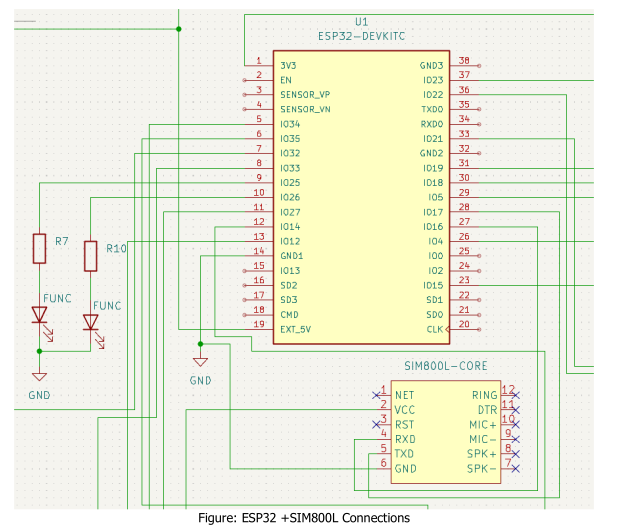
\includegraphics[width=0.85\textwidth]{images/schematic-esp32-sim.png}
    \caption{ESP32-DEVKITC and SIM800L cellular module connections: UART, level-shift resistors R7--R10, and status LEDs.}
    \label{fig:schematic-esp32-sim}
\end{figure}

The ESP32 UART1 (GPIO 16/17) connects to the SIM800L module through resistors R7--R10, which form a 2~k$\Omega$ voltage divider on each line to shift the 3.3~V ESP32 logic down to the 1.8~V interface level required by the SIM800L. LEDs D2 and D5, connected through current-limiting resistors, provide visual indication of firmware operating state: D2 pulses on each CAN frame received, and D5 lights during an active GPRS transmission.

\begin{figure}[H]
    \centering
    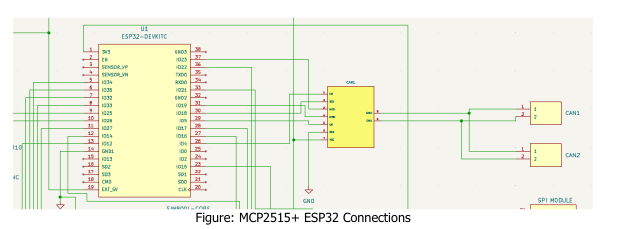
\includegraphics[width=\textwidth]{images/schematic-can.png}
    \caption{MCP2515 SPI CAN controller and TJA1051T transceiver connection detail including ESD Zener diodes D3, D4, D7.}
    \label{fig:schematic-can}
\end{figure}

The MCP2515 SPI module is connected to the ESP32 VSPI bus (SCK, MISO, MOSI) with a dedicated Chip Select line, allowing up to three independent CAN controllers to share the same SPI bus using separate CS signals. The TJA1051T transceiver converts the 3.3~V MCP2515 logic into the $\pm$2~V differential CAN\_H/CAN\_L bus signals required by the ISO~11898 physical layer standard. Zener diodes D3, D4, and D7 clamp any transient voltage spike on the CAN bus lines to safe levels before they reach the transceiver input pins.

\begin{figure}[H]
    \centering
    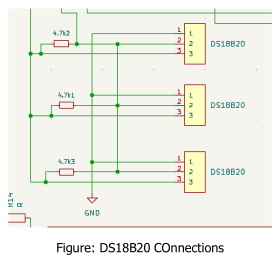
\includegraphics[width=0.55\textwidth]{images/schematic-ds18b20.png}
    \caption{Three DS18B20 temperature sensor connections (J6, J7, J8) with 4.7~k$\Omega$ 1-Wire pull-up resistors.}
    \label{fig:schematic-ds18b20}
\end{figure}

All three DS18B20 sensors share a single 1-Wire data line, which is pulled up to 3.3~V through one of the 4.7~k$\Omega$ resistors. Each sensor is factory-programmed with a unique 64-bit ROM address, allowing the ESP32 firmware to address them individually on the shared bus using the \texttt{DallasTemperature} library without any additional hardware. The three connectors (J6, J7, J8) are positioned at the board periphery so that the sensor cables can exit directly towards the motor, MPPT heatsink, and DC/DC converter mounting points.

\begin{figure}[H]
    \centering
    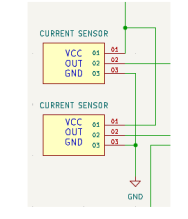
\includegraphics[width=0.45\textwidth]{images/schematic-sensors-current.png}
    \caption{Current sensor inputs: two ACS712 modules connected at J11 and J16 with analogue signal conditioning resistors.}
    \label{fig:schematic-sensors}
\end{figure}

Each ACS712 module produces an analogue output voltage centred at $V_{CC}/2$ (1.65~V) at zero current, shifting linearly at 66~mV/A for the 30~A variant used here. The signal conditioning resistors R3--R6 and R11--R14 provide a low-pass fiGPRSring and biasing network that suppresses high-frequency switching noise from the MPPT controller before the signal reaches the ESP32 ADC input, ensuring accurate current readings under electrically noisy vehicle conditions.

\begin{figure}[H]
    \centering
    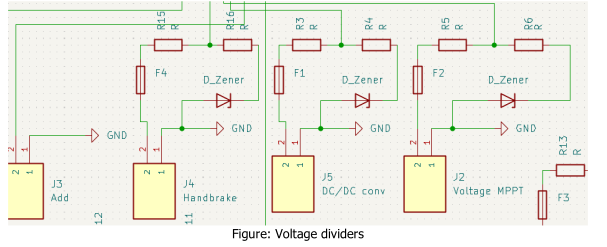
\includegraphics[width=\textwidth]{images/schematic-sensors-voltage.png}
    \caption{Voltage monitoring and auxiliary connectors: MPPT voltage divider (J2), DC/DC converter (J5), handbrake input (J4), auxiliary expansion (J3), with Zener clamp diodes D3, D4, D7 and signal conditioning resistors.}
    \label{fig:schematic-voltage-div}
\end{figure}

The MPPT output voltage, which can reach up to 50~V, is scaled down to the ESP32 ADC safe input range (0--3.3~V) using a resistive voltage divider. The Zener diodes D3, D4, and D7 clamp the ADC input line to prevent any overvoltage transient from damaging the ESP32's internal analogue circuitry. The handbrake connector J4 routes the digital handbrake signal through a pull-up resistor to a standard digital GPIO input, and the auxiliary connector J3 provides four uncommitted GPIO-connected pads for future sensor expansion.

The circuit schematic represents the logical connections between all electronic components before they are translated into physical copper traces on the PCB. The design is organised around five functional blocks.

The \textbf{ESP32-DEVKITC} (U1) is the central processing unit. It interfaces with the SIM800L cellular module (U2, using the SIM800L-CORE footprint) over UART for GPRS telemetry. The 2~k$\Omega$ resistors R7--R10 serve as UART voltage-level dividers between the 3.3~V ESP32 and the module's interface pins, protecting both ICs from logic-level mismatches. Functional status LEDs D2 and D5 indicate active operation states.

The \textbf{CAN subsystem} connects the MCP2515 SPI module to the ESP32 via SPI (Chip Select, MOSI, MISO, SCK lines), with individual chip-select pins allowing independent addressing of each CAN channel. The physical CAN layer is handled by the TJA1051T transceiver (CAN1 footprint), which interfaces with the primary CAN connector J1. A secondary CAN connector J10 provides a redundant bus connection. Zener diodes D3, D4, and D7 provide ESD and overvoltage clamping on the CAN bus lines. The 4.7~k$\Omega$ resistors (4.7k1, 4.7k2, 4.7k3) serve as bus pull-ups.

The \textbf{temperature sensing subsystem} accommodates three DS18B20 digital sensors connected via 1-Wire protocol through connectors J6, J7, and J8. The 4.7~k$\Omega$ resistors provide the mandatory pull-up on the 1-Wire data line.

The \textbf{analogue sensor subsystem} routes two current sensor inputs through J11 and J16, with signal conditioning resistors R3--R6 and R11--R14 adapting the sensor output levels to the ESP32 ADC input range. Voltage monitoring from the MPPT controller is received through J2. The handbrake digital signal is acquired through J4, providing vehicle state context for the supervision logic. Auxiliary expansion is available via connector J3.

The \textbf{protection layer} is integrated throughout the schematic. Reverse polarity protection is implemented at the main power input using diode D6. Overvoltage and ESD protection on the CAN bus is provided by Zener diodes D3, D4, and D7. Fuses F1, F2, and F3 provide overcurrent protection for the main power rail, sensor supplies, and auxiliary circuits respectively. The resistor network throughout the board ensures correct voltage levels at every inter-IC interface, preventing damage from logic-level mismatches.

\subsection{PCB Layout \& Design}

\begin{figure}[H]
    \centering
    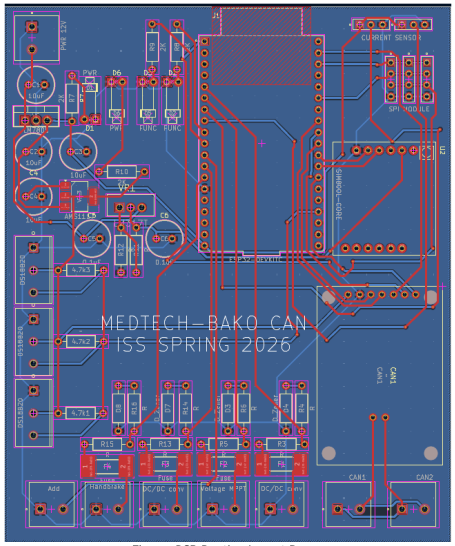
\includegraphics[width=0.75\textwidth]{images/pcb-routing.png}
    \caption{ISS board PCB routing layout (KiCad PCBnew, Rev.~RECTIFICATION\_2) showing F.Cu signal traces and B.Cu ground plane.}
    \label{fig:pcb-routing}
\end{figure}

The routing view shows all copper traces on the F.Cu (signal) layer in red and the B.Cu (ground plane) in blue. Short, direct routing of the SPI traces between the ESP32 and the MCP2515 modules minimises propagation delay and parasitic capacitance on the high-speed clock line (up to 10~MHz). Power traces carrying the 12~V input and 5~V CAN supply rails are given twice the width of signal traces to handle the required current without excessive resistive voltage drop.

\begin{figure}[H]
    \centering
    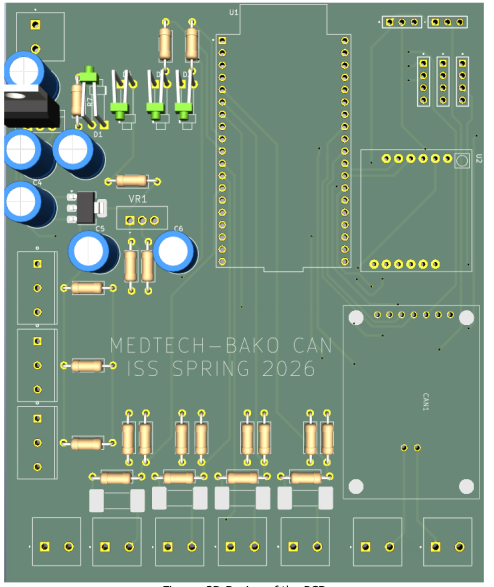
\includegraphics[width=0.75\textwidth]{images/pcb-3d.png}
    \caption{3D render of the ISS board (KiCad 3D viewer) showing component placement and board outline.}
    \label{fig:pcb-3d}
\end{figure}

The 3D render confirms correct physical clearances between tall components (electrolytic capacitors, SIM800L module, ESP32 devkit) and the board outline. The functional zoning is visible in the render: the power block occupies the top-right corner, the ESP32 and SIM800L module occupy the board centre, and the sensor connectors are distributed along the three remaining edges for clean harness routing. The board outline dimensions are compatible with a standard 100~mm $\times$ 100~mm DIN-rail enclosure footprint.

The PCB was designed using KiCad 10.0 PCBnew. Table~\ref{tab:pcb-params} summarises the key mechanical and electrical parameters of the board as extracted from the KiCad project file.

\begin{table}[H]
\centering
\caption{PCB Mechanical and Electrical Parameters}
\label{tab:pcb-params}
\begin{tabular}{>{\bfseries}p{4.2cm} p{8.0cm}}
\toprule
Parameter & Value \\
\midrule
Board title      & MONITORING SYSTEM BAKO MOTORS \\
Design revision  & RECTIFICATION\_2 (06 April 2026) \\
Layer count      & 2 layers (F.Cu + B.Cu) \\
Board thickness  & 1.6~mm \\
Copper thickness & 35~\textmu m (1~oz) per layer \\
Substrate material & FR-4 ($\varepsilon_r = 4.5$, loss tangent = 0.02) \\
Solder mask      & Both sides (front + back), 10~\textmu m \\
Silkscreen       & Front + Back \\
Min. track/spacing & Per KiCad DRC defaults \\
Via tenting      & Both sides \\
Design tool      & KiCad 10.0 / PCBnew \\
\bottomrule
\end{tabular}
\end{table}

With the two-layer stackup, the front copper layer (F.Cu) carries the majority of signal traces and component connections. The back copper layer (B.Cu) is used for the ground plane pour and power return paths, reducing electromagnetic interference and providing a low-impedance ground reference for all circuits. Critical high-frequency SPI traces connecting the ESP32 to the MCP2515 modules are kept short and routed on F.Cu to minimise parasitic inductance. Power traces carrying the 12~V input, 5~V CAN rail, and 3.3~V logic rail are given increased width to handle the required current without excessive resistive heating. Sensor signal traces, particularly the 1-Wire bus and analogue current-sense lines, are routed away from the switching regulator to avoid noise coupling.

The component placement follows a functional zoning approach to minimise cross-interference between the power, digital, and analogue sections of the board:

\begin{itemize}
    \item \textbf{Power zone:} The main power input connector (J9), fuses (F1--F3), LM2596S-ADJ (VR1), LM7805 (V5), and AMS1117 (V3.3) are grouped together to contain high-current paths and facilitate efficient heat dissipation.
    \item \textbf{Digital processing zone:} The ESP32-DEVKITC (U1) and SIM800L cellular module (U2) are placed centrally, minimising trace lengths to the SPI, UART, and GPIO peripherals.
    \item \textbf{CAN bus zone:} The MCP2515 SPI modules (J17--J19), TJA1051T transceiver, and CAN connectors (J1, J10) are grouped together at one edge of the board, simplifying external wiring harness routing to the vehicle OBD port~\cite{bakowiring}.
    \item \textbf{Sensor zone:} The DS18B20 connectors (J6--J8), current sensor inputs (J11, J16), and MPPT voltage input (J2) are placed at the board periphery, allowing sensor cables to exit cleanly without routing over the digital core.
\end{itemize}

The design was verified using KiCad's Design Rule Check (DRC) prior to export. Pad-to-mask clearance is set to 0~mm (controlled by the manufacturer's solder mask process). Via tenting is applied on both the front and back layers to prevent solder bridges and improve board reliability. The silk screen layers carry component reference designators and polarity markers to facilitate assembly and inspection. The board is ready for submission to a PCB fabrication house using standard Gerber RS-274X export from KiCad.

\subsection{Full Components Inventory}
\label{sec:components-inventory}

Tables~\ref{tab:bom-ics} and~\ref{tab:bom-passives} list all components populated on the ISS board as extracted from the KiCad PCB file (test2.kicad\_pcb, Rev.~RECTIFICATION\_2). References, values, quantities, and functional roles are provided for each entry.

\begin{table}[H]
\centering
\caption{Full Component Inventory --- Integrated Circuits and Connectors}
\label{tab:bom-ics}
\small
\begin{tabular}{>{\bfseries}p{2.4cm} p{3.2cm} c p{5.8cm}}
\toprule
Ref. & Component / Value & Qty & Function \\
\midrule
U1           & ESP32-DEVKITC        & 1 & Main MCU --- Wi-Fi, BT, UART to SIM800L \\
U2           & SIM800L-CORE*        & 1 & GPRS cellular module (SIM800L footprint) \\
V3.3         & AMS1117 (3.3\,V)     & 1 & 3.3\,V LDO for ESP32 I/O \\
V5           & LM7805               & 1 & 5\,V linear reg. for CAN side \\
VR1          & LM317T               & 1 & Adjustable voltage ref. / LM2596S-ADJ compatible \\
J1           & CAN1 connector       & 1 & Primary CAN bus interface \\
J10          & CAN2 connector       & 1 & Secondary / redundant CAN bus \\
J19/J17/J18  & SPI MODULE           & 3 & MCP2515 CAN controller via SPI \\
J11/J16      & CURRENT SENSOR       & 2 & Analogue current-sense inputs \\
J6/J7/J8     & DS18B20              & 3 & 1-Wire temperature sensors \\
J2           & Voltage MPPT         & 1 & MPPT voltage monitoring input \\
J4           & Handbrake            & 1 & Handbrake digital signal input \\
J5/J12       & DC/DC conv.          & 2 & Power conversion headers (LM2596S-ADJ) \\
J9           & PWR 12V              & 1 & 12\,V main power input connector \\
J3           & Add                  & 1 & Auxiliary / expansion connector \\
CAN1         & CAN transceiver      & 1 & TJA1051T CAN bus transceiver \\
F1/F2/F3     & Fuse                 & 3 & Overcurrent protection \\
D1           & PWR LED              & 1 & Power-on indicator \\
D2/D5        & FUNC LED             & 2 & Status / function indicators \\
D3/D4/D7     & D\_Zener             & 3 & Zener clamp / ESD protection \\
D6           & PWR diode            & 1 & Reverse-polarity / flyback protection \\
\bottomrule
\end{tabular}
\end{table}

\begin{table}[H]
\centering
\caption{Full Component Inventory --- Passive Components}
\label{tab:bom-passives}
\small
\begin{tabular}{>{\bfseries}p{2.4cm} p{3.2cm} c p{5.8cm}}
\toprule
Ref. & Component / Value & Qty & Function \\
\midrule
C1/C2/C3/C4 & 10~\textmu F cap       & 4 & Bulk decoupling capacitors \\
C5/C6        & 0.1~\textmu F cap      & 2 & High-freq. bypass capacitors \\
R7/R8/R9/R10 & 2~k$\Omega$ resistor & 4 & UART voltage-level dividers \\
4.7k1/2/3    & 4.7~k$\Omega$        & 3 & 1-Wire pull-up resistors (DS18B20) \\
R3/R5/R6, R11--R14 & Resistor (misc) & 7 & Signal conditioning \& biasing \\
R4           & 2~k$\Omega$          & 1 & UART/SIM interface level divider \\
\bottomrule
\end{tabular}
\end{table}

\noindent\small{* The SIM800L-CORE footprint reference in KiCad is used as the physical placeholder for the SIM800L module during layout. The component actually populated on the board is the SIM800L as justified in Section~6.1.}

\subsection{Component Photographs}
\label{sec:component-photos}

The photographs below show the physical components used to populate the ISS board prototype. Each image is accompanied by the reference designator and the role it fulfils in the circuit.

\begin{figure}[H]
\centering
\begin{minipage}[t]{0.30\textwidth}
    \centering
    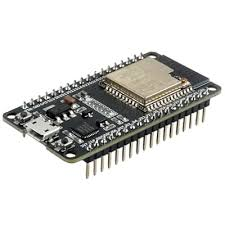
\includegraphics[width=\linewidth]{images/esp32.jpeg}
    \caption{ESP32-DEVKITC~V1 microcontroller. Central processing unit for CAN decoding, sensor acquisition, and GPRS telemetry.}
    \label{fig:photo-esp32}
\end{minipage}\hfill
\begin{minipage}[t]{0.30\textwidth}
    \centering
    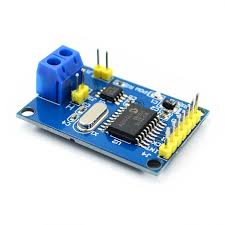
\includegraphics[width=\linewidth]{images/mcp2515.jpeg}
    \caption{MCP2515 SPI CAN controller module. Interfaces the ESP32 to the J1939 CAN bus via SPI (J17/J18/J19).}
    \label{fig:photo-mcp2515}
\end{minipage}\hfill
\begin{minipage}[t]{0.30\textwidth}
    \centering
    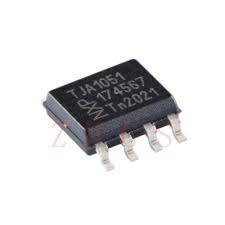
\includegraphics[width=\linewidth]{images/tja1051t.jpeg}
    \caption{TJA1051T automotive CAN transceiver. Converts MCP2515 logic levels to differential CANH/CANL bus signals.}
    \label{fig:photo-tja1051}
\end{minipage}
\end{figure}

\begin{figure}[H]
\centering
\begin{minipage}[t]{0.30\textwidth}
    \centering
    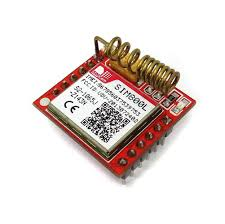
\includegraphics[width=\linewidth]{images/sim800l.jpeg}
    \caption{SIM800L GPRS Cat-M1 module. Provides 4G cellular connectivity to the VPS cloud backend via GPRS/GPRS.}
    \label{fig:photo-SIM800L}
\end{minipage}\hfill
\begin{minipage}[t]{0.30\textwidth}
    \centering
    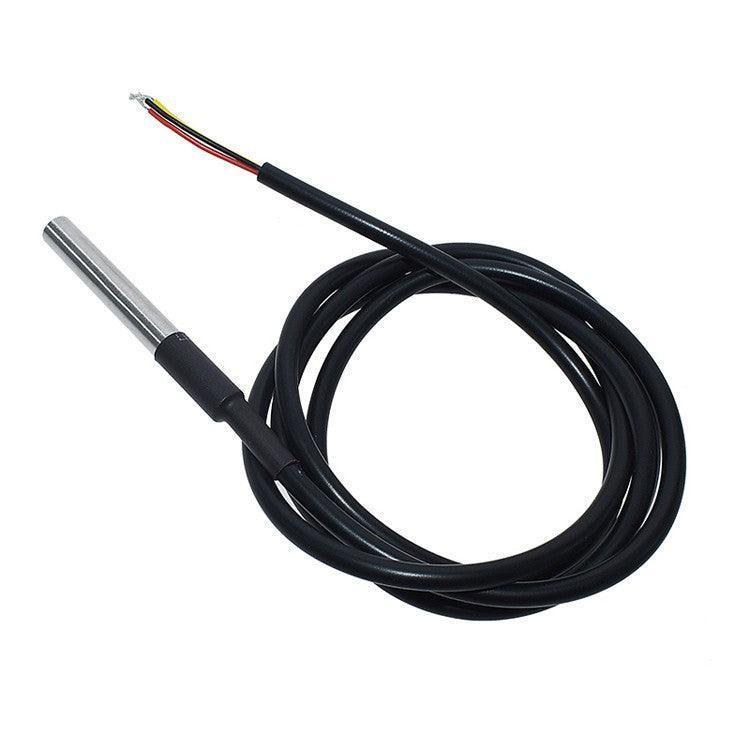
\includegraphics[width=\linewidth]{images/ds18b20-sonde-de-temperature-inoxydable-tuni-smart-innovation.jpg}
    \caption{DS18B20 1-Wire digital temperature sensors (J6, J7, J8). Monitor motor winding, MPPT heatsink, and DC/DC temperatures.}
    \label{fig:photo-ds18b20}
\end{minipage}\hfill
\begin{minipage}[t]{0.30\textwidth}
    \centering
    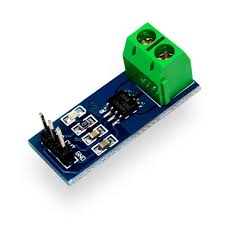
\includegraphics[width=\linewidth]{images/ACS712-30A.jpeg}
    \caption{ACS712-30A Hall-effect current sensor modules (J11, J16). Measure solar panel and MPPT output currents.}
    \label{fig:photo-acs712}
\end{minipage}
\end{figure}

\subsection{Design Summary}

The electronic design of the BAKO Motors ISS board is built around a carefully selected set of components that maximise functionality while remaining practical and cost-effective in the Tunisian market context. The ESP32 provides a powerful, affordable, and well-supported processing core. The MCP2515 and TJA1051T together form a robust, proven CAN bus interface fully compatible with the J1939 protocol used by the O'CELL BMS. The SIM800L ensures long-term GPRS network compatibility with local Tunisian operators, making it a future-proof choice over the 2G-only SIM800L. The LM2596S-ADJ provides efficient switching power conversion for the full board from the vehicle's 12~V rail.

The two-layer KiCad PCB design translates these component choices into a compact, well-organised board with clear functional zoning, adequate protection circuitry, and a layout strategy designed to minimise signal interference between the power, digital, and analogue domains. The design is at revision RECTIFICATION\_2, reflecting iterative refinement based on functional testing and layout optimisation. The board is ready for Gerber export and submission to a PCB fabrication house.
